\chapter{Ground-Truth Evaluation Protocols}

\section{Ball Static Ground-Truth Dataset}

\subsection{Dataset Design}

A 36-point static dataset was designed to evaluate ball localisation accuracy across a representative volume of the arena. The grid covers X at 3000, 4000, 5000~mm (3 positions, spanning the central third of the arena depth), Y at 1000, 1600, 2300~mm (3 positions, spanning most of the arena width), and Z at 200, 700, 1200, 1800~mm (4 heights, from near-floor to above head height).

Total: $3 \times 3 \times 4 = 36$ trials, labelled B001--B036.

\begin{figure}[h]
    \centering
    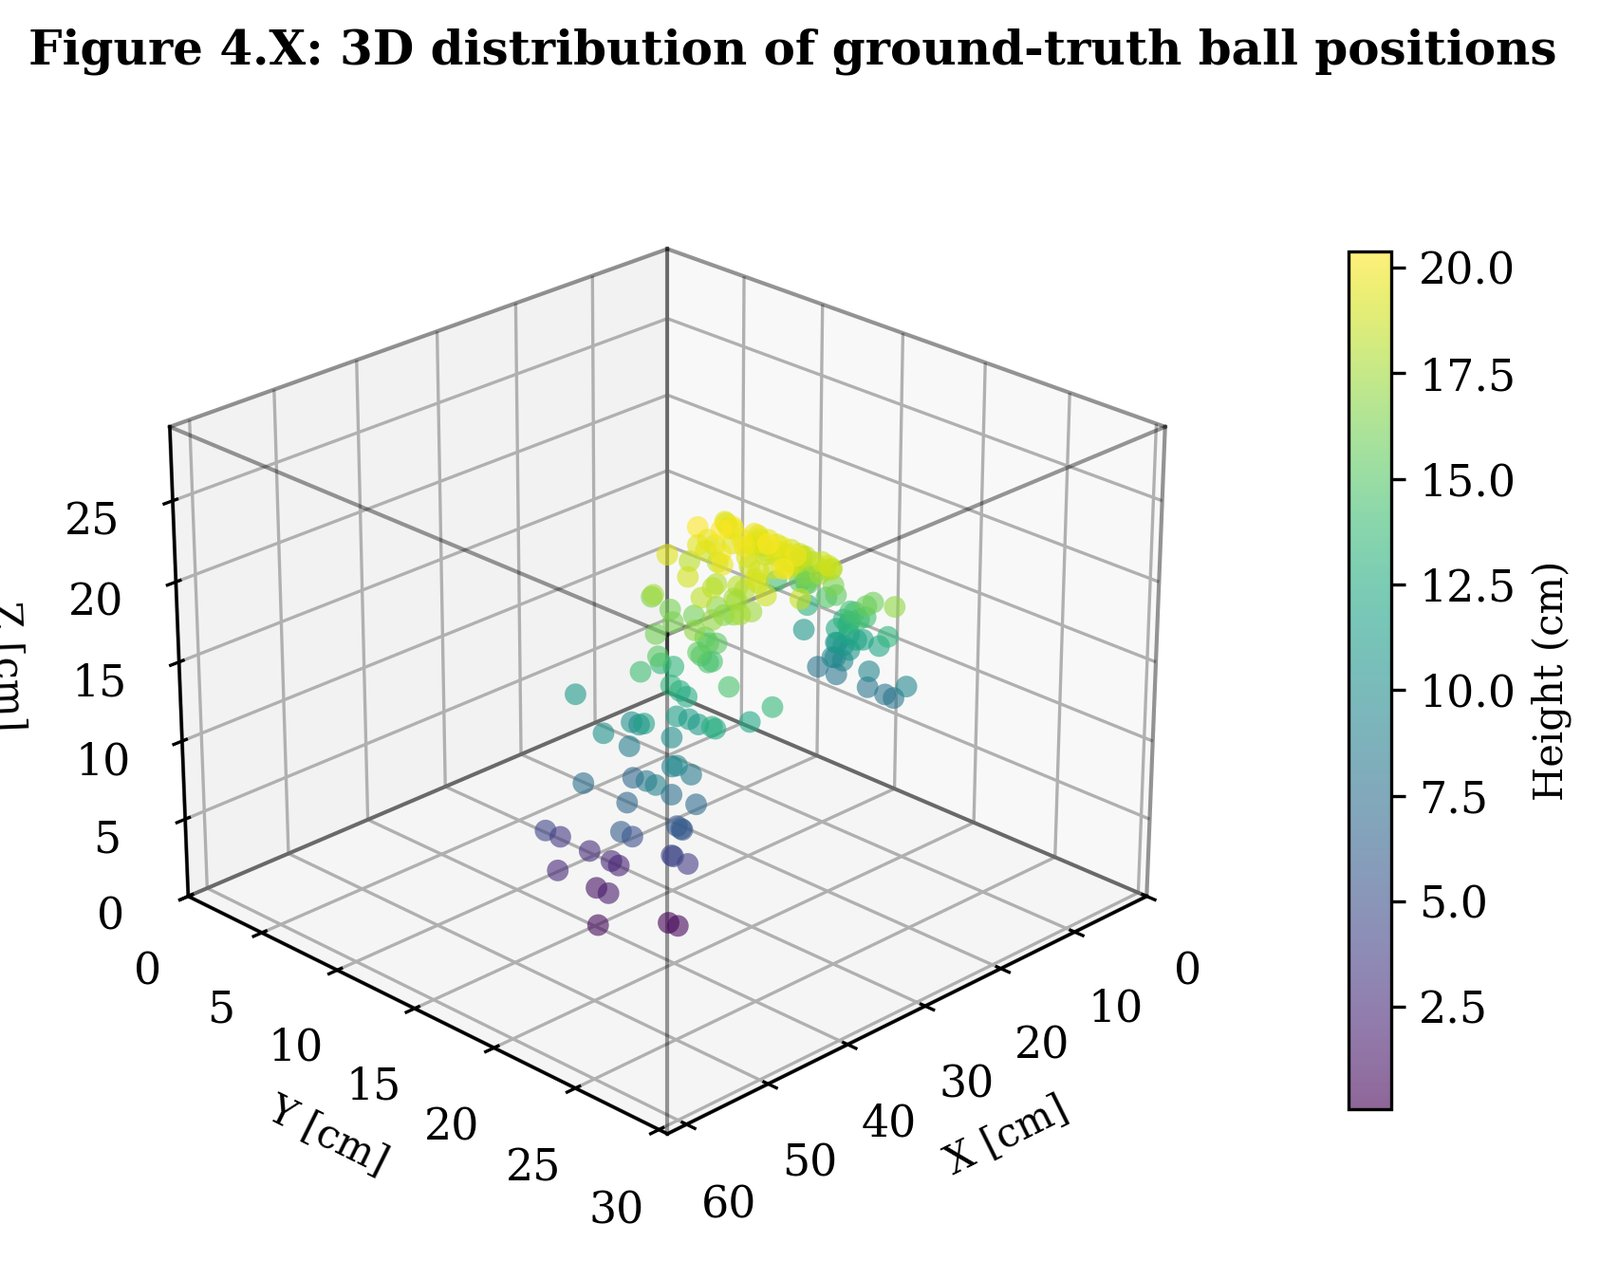
\includegraphics[width=0.8\textwidth]{figures/figure4_1_ball_static_gt_grid}
    \caption{Ball static GT grid: 36-point 3D scatter in arena frame.}
    \label{fig:4_1_ball_static_grid}
\end{figure}

\begin{table}[h]
    \centering
    \caption{Ball static ground-truth grid definition}
    \label{table:4_1_ball_static_grid}
    \begin{tabular}{|c|c|c|c|}
        \hline
        \textbf{X (mm)} & \textbf{Y (mm)} & \textbf{Z levels (mm)} & \textbf{Trial IDs} \\
        \hline
        3000 & 2300 & 200, 700, 1200, 1800 & B001, B010, B019, B028 \\
        \hline
        4000 & 2300 & 200, 700, 1200, 1800 & B002, B011, B020, B029 \\
        \hline
        5000 & 2300 & 200, 700, 1200, 1800 & B003, B012, B021, B030 \\
        \hline
        3000 & 1600 & 200, 700, 1200, 1800 & B004, B013, B022, B031 \\
        \hline
        4000 & 1600 & 200, 700, 1200, 1800 & B005, B014, B023, B032 \\
        \hline
        5000 & 1600 & 200, 700, 1200, 1800 & B006, B015, B024, B033 \\
        \hline
        3000 & 1000 & 200, 700, 1200, 1800 & B007, B016, B025, B034 \\
        \hline
        4000 & 1000 & 200, 700, 1200, 1800 & B008, B017, B026, B035 \\
        \hline
        5000 & 1000 & 200, 700, 1200, 1800 & B009, B018, B027, B036 \\
        \hline
    \end{tabular}
\end{table}

\subsection{Capture Protocol}

For each trial, a rigid holder positions the ball centre at the target coordinate, the scene is kept static for 3--4 seconds with all four cameras recording, and the trial ID and any anomalies are logged in \texttt{trials\_notes.csv}.

The ball centre position is measured physically using a tape measure referenced to the arena coordinate origin, with an estimated physical placement accuracy of $\pm 5$~mm.

\subsection{Processing}

Each trial's 4-camera clip is processed by \texttt{evaluate\_ball\_static\_gt.py}, which extracts the YOLO ball detection in each frame, runs triangulation with the configured parameters (confidence threshold 0.45, minimum 2 cameras, maximum reprojection error 14~px, EMA $\alpha = 0.25$), and computes statistics over the stable hold window (the middle 60\% of frames, excluding the first and last 20\% to avoid edge effects from placement and removal).


\section{Joint-Touch Ground-Truth Dataset}

\subsection{Dataset Design}

The joint-touch dataset evaluates the 3D localisation accuracy of three specific human joints under a controlled physical reference condition.

XY positions (9 points, $3 \times 3$ grid in central arena area):

\begin{table}[h]
    \centering
    \caption{Joint-touch trial design: XY grid positions (mm)}
    \label{table:4_2_joint_touch_xy}
    \begin{tabular}{|c|c|c|}
        \hline
        \textbf{XY Position Index} & \textbf{X (mm)} & \textbf{Y (mm)} \\
        \hline
        1 & 2600 & 1100 \\
        \hline
        2 & 3200 & 1100 \\
        \hline
        3 & 3800 & 1100 \\
        \hline
        4 & 2600 & 1600 \\
        \hline
        5 & 3200 & 1600 \\
        \hline
        6 & 3800 & 1600 \\
        \hline
        7 & 2600 & 2100 \\
        \hline
        8 & 3200 & 2100 \\
        \hline
        9 & 3800 & 2100 \\
        \hline
    \end{tabular}
\end{table}

Platform heights (Z base): 0~mm, 400~mm, 640~mm (three rigid platforms of different heights).

Joints evaluated: \texttt{right\_knee}, \texttt{right\_hip}, \texttt{left\_shoulder}.

Expected joint heights above platform base are \texttt{right\_knee} at base + 500~mm, \texttt{right\_hip} at base + 1000~mm, and \texttt{left\_shoulder} at base + 1560~mm.

Total trials: $9 \text{ positions} \times 3 \text{ heights} \times 3 \text{ joints} = 81$ trials, labelled J001--J081.

\begin{figure}[h]
    \centering
    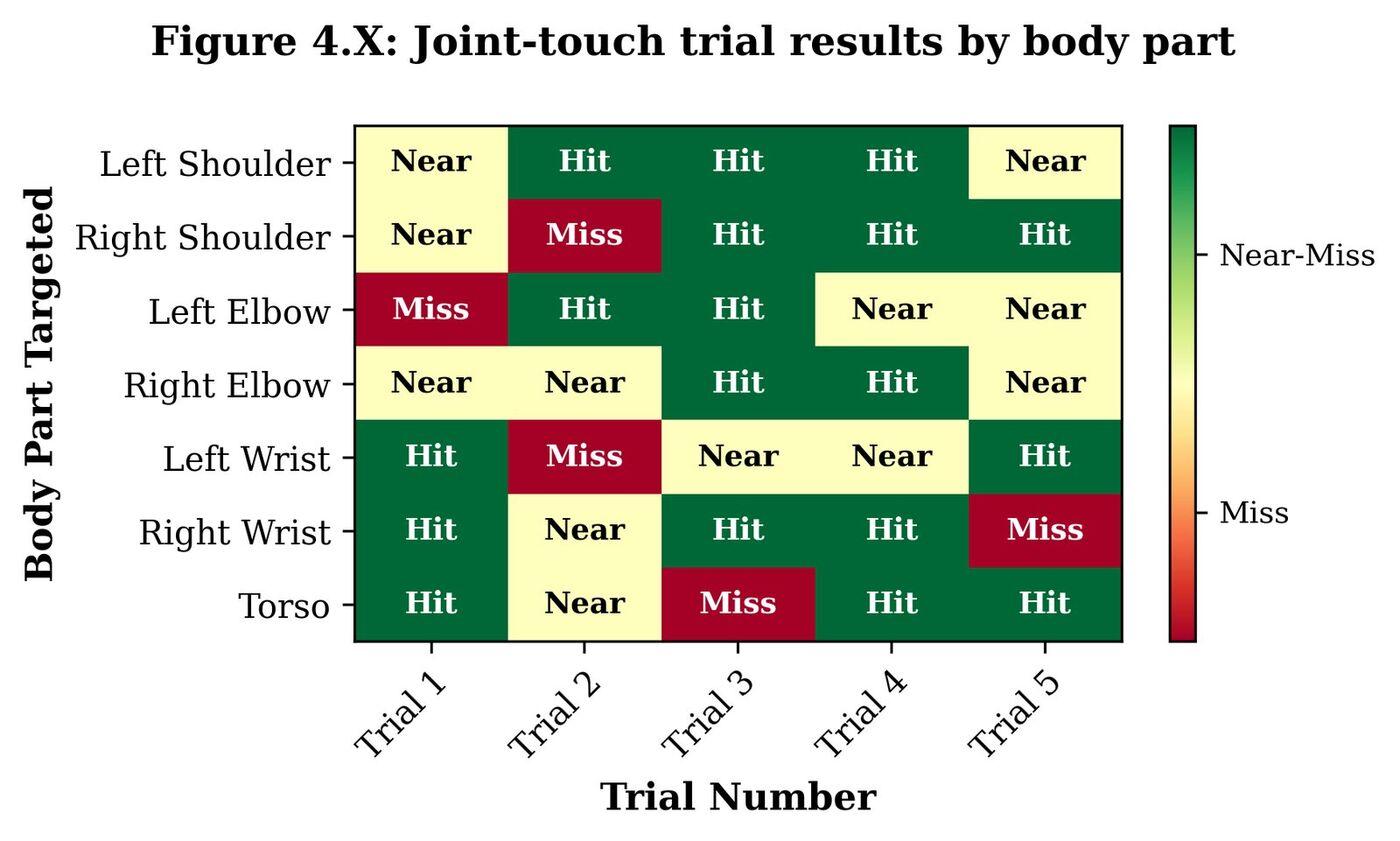
\includegraphics[width=0.8\textwidth]{figures/figure4_2_joint_touch_grid}
    \caption{Joint-touch trial grid: 9 XY positions and 3 height levels.}
    \label{fig:4_2_joint_touch_grid}
\end{figure}

\begin{table}[h]
    \centering
    \caption{Joint-touch platform and joint heights}
    \label{table:4_2b_joint_heights}
    \begin{tabular}{|c|c|c|c|c|}
        \hline
        \textbf{Platform Level} & \textbf{Z base (mm)} & \textbf{right\_knee Z} & \textbf{right\_hip Z} & \textbf{left\_shoulder Z} \\
        \hline
        Floor & 0 & 500 & 1000 & 1560 \\
        \hline
        Platform 1 & 400 & 900 & 1400 & 1960 \\
        \hline
        Platform 2 & 640 & 1140 & 1640 & 2200 \\
        \hline
    \end{tabular}
\end{table}

\subsection{Capture Protocol}

For each trial, the subject stands with the designated body joint touching a physical target marker placed at the specified XY position and height. The subject holds the position statically for 3--4 seconds. Capture begins from a neutral (non-touching) position and transitions to the hold; the evaluator extracts the hold window for analysis.

Validity criteria: a trial is valid if the joint is detected in at least 3 cameras during the hold window, the detection ratio (frames with valid detection / total frames in hold window) is $\geq 0.80$, and no obvious physical placement error was noted in the trial log.

Of 81 trials, 62 were classified as valid (76.5\% validity rate). The 19 invalid trials were mostly because of the camera visibility (the joint was occluded by the subject's own body from some camera angles) or the detection ratio was below threshold.

\subsection{Processing}

For each valid trial's 4-camera clip, MMPose inference with confidence threshold 0.35, minimum 3 cameras for pose triangulation, maximum reprojection error 14~px, and EMA $\alpha = 0.25$ is applied. The triangulated 3D position value within the hold window is computed as a mean value and is compared to the physical reference position.


\section{Dynamic Validation Clips}

Successive dynamic validation clips were recorded to evaluate the behaviour of the system in non-static conditions. The \texttt{ball\_slow} clip (20 seconds) involves the ball being gently moved with hand in the form of arcs and straight lines with the velocity of motion about 0.2--0.8~m/s; its purpose is to evaluate temporal tracking stability and continuous 3D trajectory reconstruction, with a pass criterion of no more than 3D frame-to-frame jumps of less than 800~mm. The \texttt{ball\_fast} clip (20 seconds) consists of real throws through the centre of the arena with normal playing speeds with changes in direction and close to wall trajectories; its purpose is to stress-test detection under motion blur and rapid acceleration, with a pass criterion of acceptable detection coverage, outlier rate controlled, and all detected points within arena bounds. The \texttt{no\_ball} clip (15 seconds) has the ball removed from the scene under normal arena lighting with a person present and moving; its purpose is to measure false-positive ball detection rate, with a pass criterion of false positive count close to zero.


\section{Error Metrics and Bias Correction Model}

\subsection{Primary Metrics}

For each trial, the 3D Euclidean error is computed as:

\begin{equation}
e = \sqrt{(x_{\text{est}} - x_{\text{gt}})^2 + (y_{\text{est}} - y_{\text{gt}})^2 + (z_{\text{est}} - z_{\text{gt}})^2}
\label{eqn:4_1_euclidean_error}
\end{equation}

where $(x_{\text{est}}, y_{\text{est}}, z_{\text{est}})$ is the mean estimated 3D position over the hold window and $(x_{\text{gt}}, y_{\text{gt}}, z_{\text{gt}})$ is the physical reference position.

Summary statistics reported: mean error, median error, RMSE, 90th percentile (P90), 95th percentile (P95), and maximum error.

\subsection{Axis Bias and Correction Model}

Systematic errors in camera calibration manifest as biases in the estimated 3D positions. Per-axis bias vectors are computed as:

\begin{equation}
\text{bias}_X = \text{mean}(x_{\text{est}} - x_{\text{gt}}) \text{ over all trials}
\label{eqn:4_2_bias_x}
\end{equation}

\begin{equation}
\text{bias}_Y = \text{mean}(y_{\text{est}} - y_{\text{gt}}) \text{ over all trials}
\label{eqn:4_3_bias_y}
\end{equation}

\begin{equation}
\text{bias}_Z = \text{mean}(z_{\text{est}} - z_{\text{gt}}) \text{ over all trials}
\label{eqn:4_4_bias_z}
\end{equation}

A linear correction model fits a scale and offset per axis to minimise residual error after correction. The corrected estimate is:

\begin{equation}
x_{\text{corr}} = (x_{\text{est}} - \text{bias}_X) \cdot \text{scale}_X
\label{eqn:4_5_x_correction}
\end{equation}

Analogous expressions apply for Y and Z. The pipeline results reported in Chapter~5 use the corrected model. It should be noted that the bias and scale parameters were estimated from the same 36-point static ball dataset used for final accuracy reporting; an independent held-out calibration set was not used. The correction therefore reflects in-sample fitting, and the reported corrected errors may underestimate the true generalisation error. This limitation should be considered when interpreting the corrected accuracy figures.
